
\begin{figure}[h]
\centering
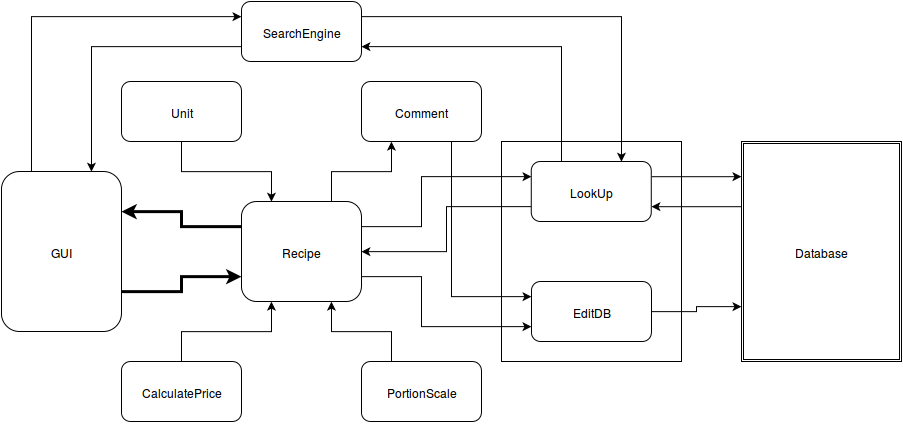
\includegraphics[scale=0.5]{overview.png}
\caption{Översikt över första lagrets moduler.}
\label{fig:overview}
\end{figure}

MatLabb har tre centrala moduler: 
\begin{enumerate}
\item En databas som lagrar all receptrelaterad information.
\item En receptmodul (\verb=Recipe=) som genom hjälpmoduler hämtar, skriver och behandlar databasens information.
\item Ett användargränssnitt (\verb=GUI=) som hjälper användaren att på ett intuitivt och välbekant sätt interagerar med receptmodulen, och i förlängningen databasen.

I detta kapitel ges en överblick över funktionaliteten hos modulerna i första ``lagret'' och hur dessa interagerar.
\end{enumerate}
